\chapter{Ausblick}

\section{Visualisierung von Wetter- und Wellendaten}
Die visuelle Darstellung der Wetterlage wäre eine weitere nützliche
Anwendung für die man die Wetter- und Wellendaten der beiden Modelle
verwenden könnte. Um einen besseren Eindruck von der Gesamtwetterlage
zu bekommen, werden in Wettersendungen im Fernsehen meist sogenannte
Strömungsfilme gezeigt. Die Wetterlage wird in diesen Filmen meist
durch unterschiedlich eingefärbte Bereiche über einer Landkarte
dargestellt. Durch das Abspielen im Zeitraffer kann man so z.B. die
Ausbreitung von Hoch- und Tiefdruckgebieten verfolgen und sich einen
besseren Überblick von der Gesamtwetterlage in den nächsten Stunden
und Tagen verschaffen. Da surfbare Wellen oft durch den viele
Kilometer weit gereisten Swell entstehen, ist eine globale Betrachtung
dessen Ausbreitung recht aufschlussreich. In Abbildung
\ref{wave-watch-grads} ist die graphische Aufbereitung der Wellenhöhe
und einiger weiterer Vorhersageelement über dem Atlantik zu sehen. Die
verschiedenen Wellenhöhen sind dort in unterschiedlichen Farben
gekennzeichnet. Spielt man mehrere, zu verschiedenen Zeitpunkten
generierte Bilder hintereinander ab, kann man die Ausbreitung der
Wellen sehr gut veranschaulichen. Durch diese Darstellung kann man
sehr gut Trends erkennen die bei einer Darstellung der Wellenhöhen in
bloßen Zahlen gar nicht auffallen würden. Betrachtet man
beispielsweise nur die Wellenhöhen an einem bestimmten Spot kann man
nur eine Aussage für die nächsten 180 Stunden machen. Zieht man jedoch
die visuelle Darstellung der Wellenausbreitung hinzu, kann man oft
einen dort erst sehr viel später eintreffenden Swell erkennen und eine
Einschätzung weit über 180 Stunden hinaus bekommen. Eine Darstellung
solche Strömungsfilme für einige ausgewählte Regionen wäre eine
wünschenswerte Erweiterung, mit der den Nutzern der Web Applikation
ein Mehrwert geboten werden könnte. Einige Webseiten
\footnote{\url{http://nomad5.ncep.noaa.gov/cgi-bin/pdisp_wave.sh}}
bieten bereits sehr gute \footnote{\url{http://magicseaweed.com}}
Aufbereitung solcher Vorhersagen an, und eine Integration eines
solchen Feature in die Web Applikation wäre ebenfalls
wünschenswert. Um Plots wie der in Abbildung \ref{wave-watch-grads}
und Strömungsfilme zu erstellen, kann das Programme \textit{Grads}
\footnote{\url{http://www.iges.org/grads/}} verwendet werden.

\begin{figure}[h]
  \begin{center}
    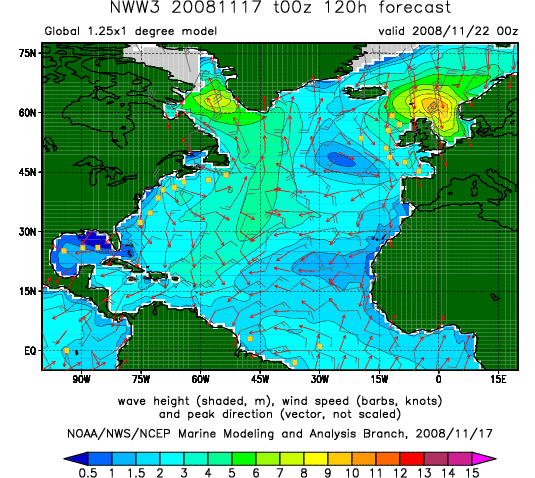
\includegraphics[width=\textwidth]{bilder/wave-watch}
    \caption{Plot einiger Elemente des Wave Watch III Modells}
    \label{wave-watch-grads}
  \end{center}
\end{figure}

\section{Verbesserung der Vorhersagen}
Die aus dem \textit{Global Forecast System} und dem \textit{Wave Watch
  III} Modell stammenden Wetter- und Wellenvorhersagen beruhen zwar
auf einem numerisch berechneten Wettermodell, können aber nur bedingt
zur Vorhersage der tatsächlichen Surfbedingungen verwendet werden. In
Kombination mit Erfahrungswerten und der Kenntnis lokaler
Gegebenheiten dienen sie eher als Indikator zur Einschätzung dieser
Bedingungen. In welcher Verbindung die Vorhersagewerte mit der
Qualität der vor Ort brechenden Wellen stehen ist unklar und variiert
wohl von Spot zu Spot. Hinzu kommt, dass wegen der groben
Gitterauflösung der Modelle die Vorhersagewerte teilweise aus der
näheren Umgebung eines Spots herangezogen werden müssen. Trotzdem sind
aber vor allem die Wellenhöhe, die Wellenperiode, die Windstärke und
die Windrichtung der Modelle wichtige Indizien, die bei der
Einschätzung der Surfbedingungen eine große Rolle spielen. Was noch
fehlt ist eine Komponente mit der die lokalen Gegebenheiten eines Surf
Spots mit ins Spiel gebracht werden. Außerdem wäre es wünschenswert
eine Aussage über die Qualität der Surfbedingungen an einem Spot
treffen zu können.

\subsubsection{Beobachtung lokaler Gegebenheiten}
Würde man die Qualität der Surfbedingungen an einem Spot mit den dort
prognostizierten Wetter- und Wellenvorhersagen über einen längeren
Zeitraum hinweg vergleichen, könnte man wahrscheinlich bestimmte
Zusammenhänge feststellen. Beispielsweise ist es durchaus üblich, dass
zwei benachbarte Spots sehr ähnlichen Wetter- und Wellenverhältnissen
ausgesetzt sind, die Qualität der brechenden Wellen sich aber
erheblich unterscheidet. Dies kann z.B. daran liegen, dass der eine
Spot besser bei Flut und der andere besser bei Ebbe bricht. Manche
Spots fangen erst bei einer bestimmten Wellenhöhe an zu brechen,
andere hingegen sind bei zu großen Wellen nicht mehr surfbar, da die
Wellen sofort in sich zusammenfallen. Vor Ort ansässige Surfer,
sogenannte \textit{Locals}, haben oft ein feines Gespühr für diese
Zusammenhänge, was wohl auf deren langjährige Beobachtungen
zurückzuführen ist.

Diese Beobachtungen von den Benutzern der Web Applikation vornehmen zu
lassen ist eher unrealistisch. Zum einen sind solche Beobachtungen
sehr aufwendig, und zum anderen müsste sichergestellt sein, dass diese
diszipliniert und nach den selben Kriterien durchgeführt werden. Zudem
stellt sich die Frage wie diese Beobachtungen maschinell verwertet und
in Verbindung mit den Vorhersagen gebracht werden können.

\subsubsection{Abstimmung durch die Benutzer}
Eine im Rahmen dieser Arbeit leider nicht weiter verfolgbare Idee,
welche diese Problematik vielleicht lösen könnte, wäre die Einführung
eines Abstimmungssystems in Kombination mit Data Mining
Verfahren. Informiert sich ein Benutzer auf der Webseite über die
Surfbedingungen an einem bestimmten Spot, könnte man ihn zu den
Bedingungen in den letzten Tagen befragen. Mit etwas Glück kann es
nämlich durchaus sein, dass der Benutzer dort surfen war und eine
Aussage über die damalige Qualität der Wellen treffen kann. Diese
Befragung sollte benutzerfreundlich und schnell von statten gehen,
damit sich die Besucher nicht belästigt fühlen sondern konstruktiv
daran teilnehmen. Hier würde sich z.B. eine Bewertungsskala von 1 bis
5 ''Sternen'' mit einer Auswahl des entsprechenden Zeitpunktes
anbieten. Die so erhobenen Datensätze sollten Informationen über den
Spot, den Zeitpunkt zu dem der Benutzer surfen war, die Qualität der
Wellen und den Benutzer selbst (optional) enthalten. Sammelt man viele
dieser Bewertungen können diese statistisch ausgewertet und eine
Aussage darüber getroffen werden, wie gut die Surfbedingungen in der
Vergangenheit waren. Mit diesen Informationen könnte man z.B. die
besten Spots in einer Region bestimmen oder die Konsistenz der
Surfbedingungen an einem Spot ermitteln. Eine weitaus interessantere
Verwendung dieser Daten wäre aber, sie für die Bewertung von
zukünftigen Surfbedingungen einzusetzen.

\subsubsection{Bewertung zukünftiger Surfbedingungen}
Es wäre wünschenswert, wenn man einem Benutzer neben den Wetter- und
Wellenvorhersagen auch noch eine Einschätzung zur Qualität der
Surfbedingungen geben könnte, in der die lokalen Gegebenheiten eines
Spots mit berücksichtigt sind. Diese Einschätzung sollte dem Benutzer
in der ihm bekannten Bewertungsskala aus dem Abstimmungssystem
präsentiert werden. Je besser die Surfbedingungen, desto mehr
''Sterne''. Der zugrunde liegende Ansatz besteht in der Vermutung,
dass ähnliche Wetter- und Wellenvorhersagen auch ähnliche
Surfbedingungen provozieren. Wurden für einen Zeitpunkt in der
Vergangenheit positive Bewertung abgegeben, sind die Surfbedingungen
zu einem zukünftigen Zeitpunkt mit ähnlichen Wetter- und
Wellenverhältnissen vielleicht auch gut, und umgekehrt. Durch den
Vergleich der historischen Vorhersagedaten mit denen der Zukunft, und
einer Strategie aus den abgegebenen Bewertungen welche für die Zukunft
vorherzusagen, könnte vielleicht zum Erfolg führen.

\subsubsection{Bewertungen als Klassifikationsproblem}
Die hier zu lösende Aufgabe ist ein sogenanntes
Klassifikationsproblem. Objekte einer Menge, deren
Klassenzugehörigkeit nicht bekannt ist, müssen dabei einer bestimmten
Klasse zugeordnet werden. Als Klassifikator bezeichnet man den
Algorithmus oder das Verfahren nach dem diese Zuordnung durchgeführt
wird. Klassen würden hier durch die in mehrere Abschnitte unterteilte
Bewertungsskala repräsentiert, Objekte durch die Vorhersagen an den
Spots. Die Bewertung der Surfbedingungen würde sich dann aus der
Klasse ergeben, der eine Vorhersage zugeordnet wurde. Wüsste man wie
sich die Variablen einer Vorhersage auf die Qualität der Wellen
auswirken, könnte man für jeden Spot einen Klassifikator konstruieren,
der idealerweise auch noch die lokalen Gegebenheiten mit
einbezieht. Die Vorschriften wie solch ein Klassifikator jedoch
konstruiert wird, sind jedoch meistens nicht bekannt, bzw. nur mit
hohem Aufwand zu ermitteln.

\subsubsection{Anwendung von Data Mining Verfahren}
Unter \textit{Data Mining} versteht man die Anwendung verschiedenster
Algorithmen auf einem Datenbestand, mit dem Ziel meist noch nicht
bekannte Muster zu entdecken. Neben vielen Anwendungsbeispielen ist in
\cite{Seagaran2007} nicht nur eine Zusammenfassung der in diesem
Gebiet häufig verwendeten Algorithmen zu finden, sondern auch eine
Diskussion über deren Vor- und Nachteile. Einige der dort
vorgestellten Algorithmen können dazu benutzt werden
Klassifikationsprobleme zu lösen, und bedienen sich Techniken aus dem
Bereich des maschinellen Lernens. Mit diesen Verfahren könnte versucht
werden die Zusammenhänge zwischen den Vorhersagen, den lokalen
Gegebenheiten und der Qualität der Surfbedingungen zu finden und
daraus zukünftige Bewertungen abzuleiten. \textit{Bayesian
  Classifier}, \textit{Decision Trees}, und \textit{Neuronale
  Netzwerke} sind nur einige der vorgestellten Algorithmen, mit denen
man versuchen könnte dieses Problem zu lösen.

\subsubsection{Supervised Learning}
Bei Algorithmen aus dem Bereich des maschinellen Lernens unterscheidet
man zwischen Verfahren des \textit{Supervised-} und
\textit{Unsupervised Learning}. Beim \textit{Supervised Learning}
werden sogenannte Trainingsdaten benötigt, die von den Algorithmen
analysiert und zur Lösung des Problems herangezogen werden. Die
Trainingsdaten für Klassifikationsprobleme bestehen dabei aus einer
Menge von Objekten, deren Klassenzugehörigkeit bekannt ist. Die durch
das Abstimmungssystem erhobenen Daten können somit nicht nur für
statistische Zwecke verwendet werden, sondern bieten sich auch als
Trainingsdaten für diese Kategorie der Algorithmen an. Die
Vorhersagedaten sind die Attribute eines Objekts, und die
Klassenzugehörigkeit wurde durch die Bewertung des Benutzers
festgelegt.

\subsubsection{Support Vector Machine}
Der unter dem Namen \textit{Support Vector Machine} bekannte
Algorithmus scheint ein viel versprechender Kandidat zu sein, um das
hier beschriebene Klassifikationsproblem anzugehen. Zum einen ist der
Algorithmus bei der Klassifikation von Objekten sehr schnell, und zum
anderen liefert er auch bei einer hohen Anzahl an Dimensionen recht
zuverlässige Ergebnisse. Als Dimension bezeichnet man die Attribute
eines zu klassifizierenden Objekts. Bei dem hier zu lösenden Problem
wären dies die Elemente einer Vorhersage und evtl. weitere bekannte
Eigenschaften eines Spots, die sich auf die Qualität der
Surfbedingungen auswirken könnten.

Um nun die Bewertungen zur Qualität der Surfbedingungen zu berechnen,
würde man für jeden Spot eine separate Instanz des Algorithmus
erzeugen und diese trainieren. Jede Instanz wird dabei nur mit
denjenigen Vorhersagedaten und Bewertungen trainiert, die auch zu dem
entsprechenden Spot gehören. Je mehr Trainingsdaten vorhanden sind
desto besser sind die Ergebnisse einer solchen Instanz. Da die
Trainingsphase aufwendiger als die eigentliche Klassifikation ist, und
bei hinzukommenden Trainingsdaten die Instanz erneut mit allen
Trainingsdaten initialisiert werden muss, bieten die meisten
Implementierungen des Algorithmus die Möglichkeit das Ergebnis der
Trainingsphase in einem sogenannten Modell zu speichern und zu laden.

Zur Berechnung einer Bewertung wird eine Vorhersage der entsprechenden
Instanz des Algorithmus übergeben, der dann das Ergebnis unter
Berücksichtigung der Trainingsdaten berechnet. Um dies Berechnung in
die Web Applikation zu integrieren würde man beispielsweise einmal
täglich für jeden Spot eine Instanz des Algorithmus mit den
zugehörigen Trainingsdaten initialisieren und persistent
abspeichern. Da die Klassifikation einer Vorhersage schnell zu
berechnen ist, könnte die Bewertung sogar bei einem Seitenaufruf der
Web Applikation dynamisch generiert werden. Alternativ könnte man die
Berechnung auch in den \textit{ETL-}Prozess integrieren, und alle
Bewertungen in der Datenbank vorhalten.

Anzumerken ist hier noch, dass der \textit{Support Vector Machine}
Algorithmus ein sogenanntes \textit{Black-Box} Verfahren ist, d.h. die
lokalen Gegebenheiten eines Spots fließen hier indirekt über die
erhobenen Abstimmungsdaten mit in die Bewertung ein. Welche
Zusammenhänge allerdings zwischen den Vorhersagedaten und den lokalen
Gegebenheiten bestehen können mit diesem Verfahren nicht ermittelt
werden.

\subsubsection{Erfolgsaussichten und Hindernisse}
Damit mit dem Algorithmus gute Ergebnisse erzielt werden können
benötigt man allerdings eine größere Menge an Trainingsdaten. Da diese
zum jetzigen Zeitpunkt nicht vorhanden sind, kann dieser Ansatz hier
leider nicht weiter verfolgt werden. Diese müssten im produktiven
Betrieb der Web Applikation über einen längeren Zeitraum durch die
Benutzern erstellt werden.

Ob dieses Verfahren überhaupt zum Ziel führt, müsste durch eine
Auswertung der Ergebnisse an verschiedenen Spots überprüft
werden. Zudem werden dem Algorithmus bei der Initialisierung noch
einige Parameter übergeben, die sich auf die Berechnung der
Bewertungen auswirken. Diese Parameter variieren von Problem zu
Problem können, aber durch ein Verfahren das sich
\textit{Crossvalidation} nennt ermittelt werden. Eine ausführliche
Auswertung und Probephase ist deshalb auf jeden Fall erforderlich, um
die Erfolgsaussichten einschätzen zu können.

Falls die Ergebnisse einer solchen Auswertung jedoch positiv
ausfallen, hätte man einen guten Weg gefunden die lokalen
Gegebenheiten eines Spots indirekt über die Trainingsdaten in die
Vorhersagen in Form einer Bewertung mit einfließen zu lassen.

%%% Local Variables:
%%% mode: latex
%%% TeX-master: "../community-plattform"
%%% End:
